
\documentclass[twocolumn,11pt]{article}
\setlength{\textheight}{9truein}
\setlength{\topmargin}{-0.9truein}
\setlength{\parindent}{0pt}
\setlength{\parskip}{10pt}
\setlength{\columnsep}{.4in}
\newcommand{\beq}{\begin{equation}}
\newcommand{\eeq}{\end{equation}}
\renewcommand{\abstractname}{Abstract}
\usepackage{graphicx}
\usepackage{url}
\title{NAEST - Experiment 01 Report \\ Density and Packing Fraction of Tiny Objects}
\author{Shuvam Banerji Seal\\2023WB00609}
\date{\today}
\usepackage{ragged2e}
\usepackage{amsmath}
\usepackage{amsfonts}
\usepackage{caption}
\usepackage{stackengine}
\usepackage{amssymb}
\usepackage{graphicx}
\usepackage{accents}
\usepackage{booktabs}
\usepackage{eqnarray}
\usepackage{url}
\usepackage{blindtext}
\usepackage{tcolorbox}
\usepackage{graphicx}   
\usepackage{amsthm}
\usepackage{algorithm}
\usepackage{hyperref}
\hypersetup{
    colorlinks=true,
    linkcolor=blue,
    filecolor=magenta,      
    urlcolor=blue,
    pdftitle={NAEST-Shuvam Banerji Seal},
    pdfpagemode=FullScreen,
    }
\usepackage{gensymb}
\usepackage{algpseudocode}
\usepackage{subcaption}
\usepackage[english]{babel}
\usepackage[export]{adjustbox}
\usepackage{enumerate}
\usepackage[left=2.5cm,right=2.5cm,top=1.5cm,bottom=1.5cm]{geometry}
\usepackage{lineno}
\usepackage{cite}
\usepackage{acronym}
\usepackage{xcolor}
\newcommand{\remark}[3]{%
    {\colorbox{#2}{\sffamily\scriptsize\bfseries\textcolor{white}{#1}}}
    {\sffamily\small\itshape\textcolor{#2}{#3}}
}

\begin{document}
\definecolor{aqua}{rgb}{0.0, 1.0, 1.0}
%\hypersetup{colorlinks,urlcolor=blue}
\pagestyle{plain}
 \twocolumn[
   \begin{@twocolumnfalse}
   \textbf{\maketitle}
   \setlength{\parindent}{0pt}
   \begin{abstract} 
   \textbf{Keywords:} experimental study, measurement methods, tiny particles, white mustard seeds, mass, density, volume, beam balance, terminal velocity, packing fraction, packing efficiency, black pepper seeds, scientific investigation, critical thinking.
\vspace{0.5cm}

This experimental study explores innovative measurement methods to determine the parameters of tiny particles, focusing on white mustard seeds as the test subject. Directly measuring properties like mass, density, and volume for such small particles presents considerable challenges. The investigation is divided into two parts: Part 1 involves a homemade beam balance using a plastic scale and two identical cups to measure the mass of the seeds relative to water volume, from which the density of the mustard seeds is calculated. Part 2 employs terminal velocity measurements in a water-filled transparent bottle to calculate the density using a specific relation that considers object radius, density, liquid density, and viscosity. The discrepancy in the densities obtained from the two methods is attributed to gaps between the seeds and less dense air present in Part 1. The packing fraction, representing the ratio of actual volume to occupied volume, is calculated from the density difference. The study demonstrates a packing efficiency of 65.34\% based on Part 1 data, 64.306\% based on radius and number of seeds, and 94.5\% based on 2D packing. Additionally, black pepper seeds were used to perform similar experiments, resulting in a packing efficiency of 49.67\% based on density difference, 53.85\% based on radius and number of seeds, and 78.39\% based on 2D packing. The experiment highlights the challenges and importance of accurate measurements for tiny particles, providing valuable insights for future scientific investigations and fostering critical thinking in scientific exploration.

		\vspace{.3in} 
     \end{abstract}
    \end{@twocolumnfalse}]

\section{Introduction}
In this experiment, we aim to measure the parameters of tiny particles, specifically black mustard seeds\footnote{Actually, I wasn't able to get the black mustard seeds, so I used white mustard seeds}, which are readily available in the kitchen. Directly measuring properties like mass, density, and volume for such small particles poses considerable challenges. Thus, we will employ innovative methods to determine these parameters.
\section{Aim:}
\begin{enumerate}
    \item To find the density of the seeds
    \item To find the packing fraction of the small almost spherical seeds from the difference in their desnsities measured using two different methods
\end{enumerate}
\section{Materials Required}

To conduct this experiment, we will require the following materials:
\begin{itemize}
    \item mustard seeds
    \item Scales \footnote{I used a metal, instead of a plastic one, as that was what was available in my stuff at the hostel.}
    \item Threads
    \item Small plastic cups (such as medicine cups with graduations)
    \item Long transparent bottle (preferably 2 liters)
    \item Water
    \item Beam balance (homemade, as described in the experiment)
    \item Stopwatch or mobile with a timer function
\end{itemize}

\section{Understanding the Process}
\subsection{Part 1: Measuring the Density of the Seeds Using Beam-balance}
To find the density of the seeds, we will measure the mass of a handful of seeds occupying a known volume. We will create our own beam balance using a plastic scale and two identical small plastic cups. The balance will allow us to measure the mass accurately while keeping the scale horizontal.
\begin{enumerate}
    \item I used a 30cm long metal scale whose centre of mass(COM) was around 16.1cm mark, due to the extra length of the scale. (Click \href{https://drive.google.com/file/d/153ypuE-LtqAybvo5taYfaOPsymXNsXfZ/view?usp=drive_link}{here} for the video)
    \item This scale was then hung at the COM using a few layers of very thin thread.
    \item As the balance was too sensitive to even any wind, so an extra support using the string was added to support the balance.
    \item Them accordingly the two medicine measuring cups were added so the the level of the balance isn't disturbed.
    \item Then carefully the seeds were loaded till 2.5 cm level counting upto 477 nos. and with respect to that the water was added drop-wise till they are at equilibrium.
\end{enumerate}
\subsection{Part 2: Density from Terminal Velocity}
For objects like mustard seeds, achieving terminal velocity occurs after they have moved a few centimeters in a liquid when dropped. By considering the object's spherical shape, we can use a specific relation that depends on its radius, density, density of the liquid, and viscosity to calculate the terminal velocity.
\begin{figure}[H]
    \centering
    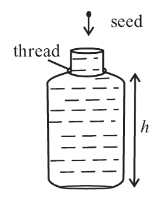
\includegraphics{part2-fig.png}
    \caption{Illustrative Diagram for the Part-2 Experiment}
    \label{Illustrative Diagram for the Part-2 Experiment}
\end{figure}
The procedure thus followed involves:
\begin{enumerate}
    \item The appropriate height at which the seeds reached their terminal velocity was eyeballed and marked on the bottle\footnote{I wasn't able to get my hands on good 2L bottles.The ones I got were terribly reflective due to inconsistency of their radii. So I used whatever I had. As the phenomenon depends on height, hopefully it should be fine.}.
    \item \textit{For better accuracy, video recording was done for the drop test and based on that video in editor, the appropriate time intervals were recorded.}
    \item Only the straight Falling seeds were taken into consideration.
\end{enumerate}
\subsection{Part 3: Calculate the Packing Fraction}
We will determine the packing fraction of the mustard seeds using the difference in densities obtained from the measurements made in the beam balance and the measurements from the terminal velocity of seeds.
\section{Calculations and Data Tabulation:}
\subsection{Part 1: Measuring the Density of the Seeds Using Beam-balance}
\subsubsection{Radius Data Table}
\begin{center}
\begin{tabular}{||c | c | c ||} 
 \hline
 SL. No. & Diameter (cm) & Radius (cm) \\ [0.5ex] 
 \hline\hline
 1 & 0.2 & 0.1 \\ 
 \hline
 2 & 0.1 & 0.05 \\
 \hline
 3 & 0.2 & 0.1 \\
 \hline
 4 & 0.2 & 0.1 \\
 \hline
 5 & 0.2 & 0.1 \\ 
 \hline
 6 & 0.2 & 0.1 \\
 \hline
  7 & 0.2 & 0.1 \\
 \hline
 8 & 0.1 & 0.05 \\
 \hline
 9 & 0.2 & 0.1 \\
 \hline
 10 & 0.3 & 0.15 \\
 \hline
 \hline
\end{tabular}
\end{center}
\\
So, Average Radius is $R_s &=  0.095 cm$\\
Number of seeds here\footnote{Yes, I counted them!! I don't know what to do with my life!} = 1343 \\

So, the volume occupied by 1343 seeds = 
\beq
\label{Volume of the seeds in the cup}
1043\times (\frac{4}{3}\pi R_s^3) = 4.823 ml
\eeq

\subsubsection{Data from Beam Balance\footnote{I was actually thinking of incorporating the packing fraction here to do a separate and more accurate calculation, but since it was also in the agenda, it will just be a simple addition thing.}}
\begin{figure}[H]
    \centering
    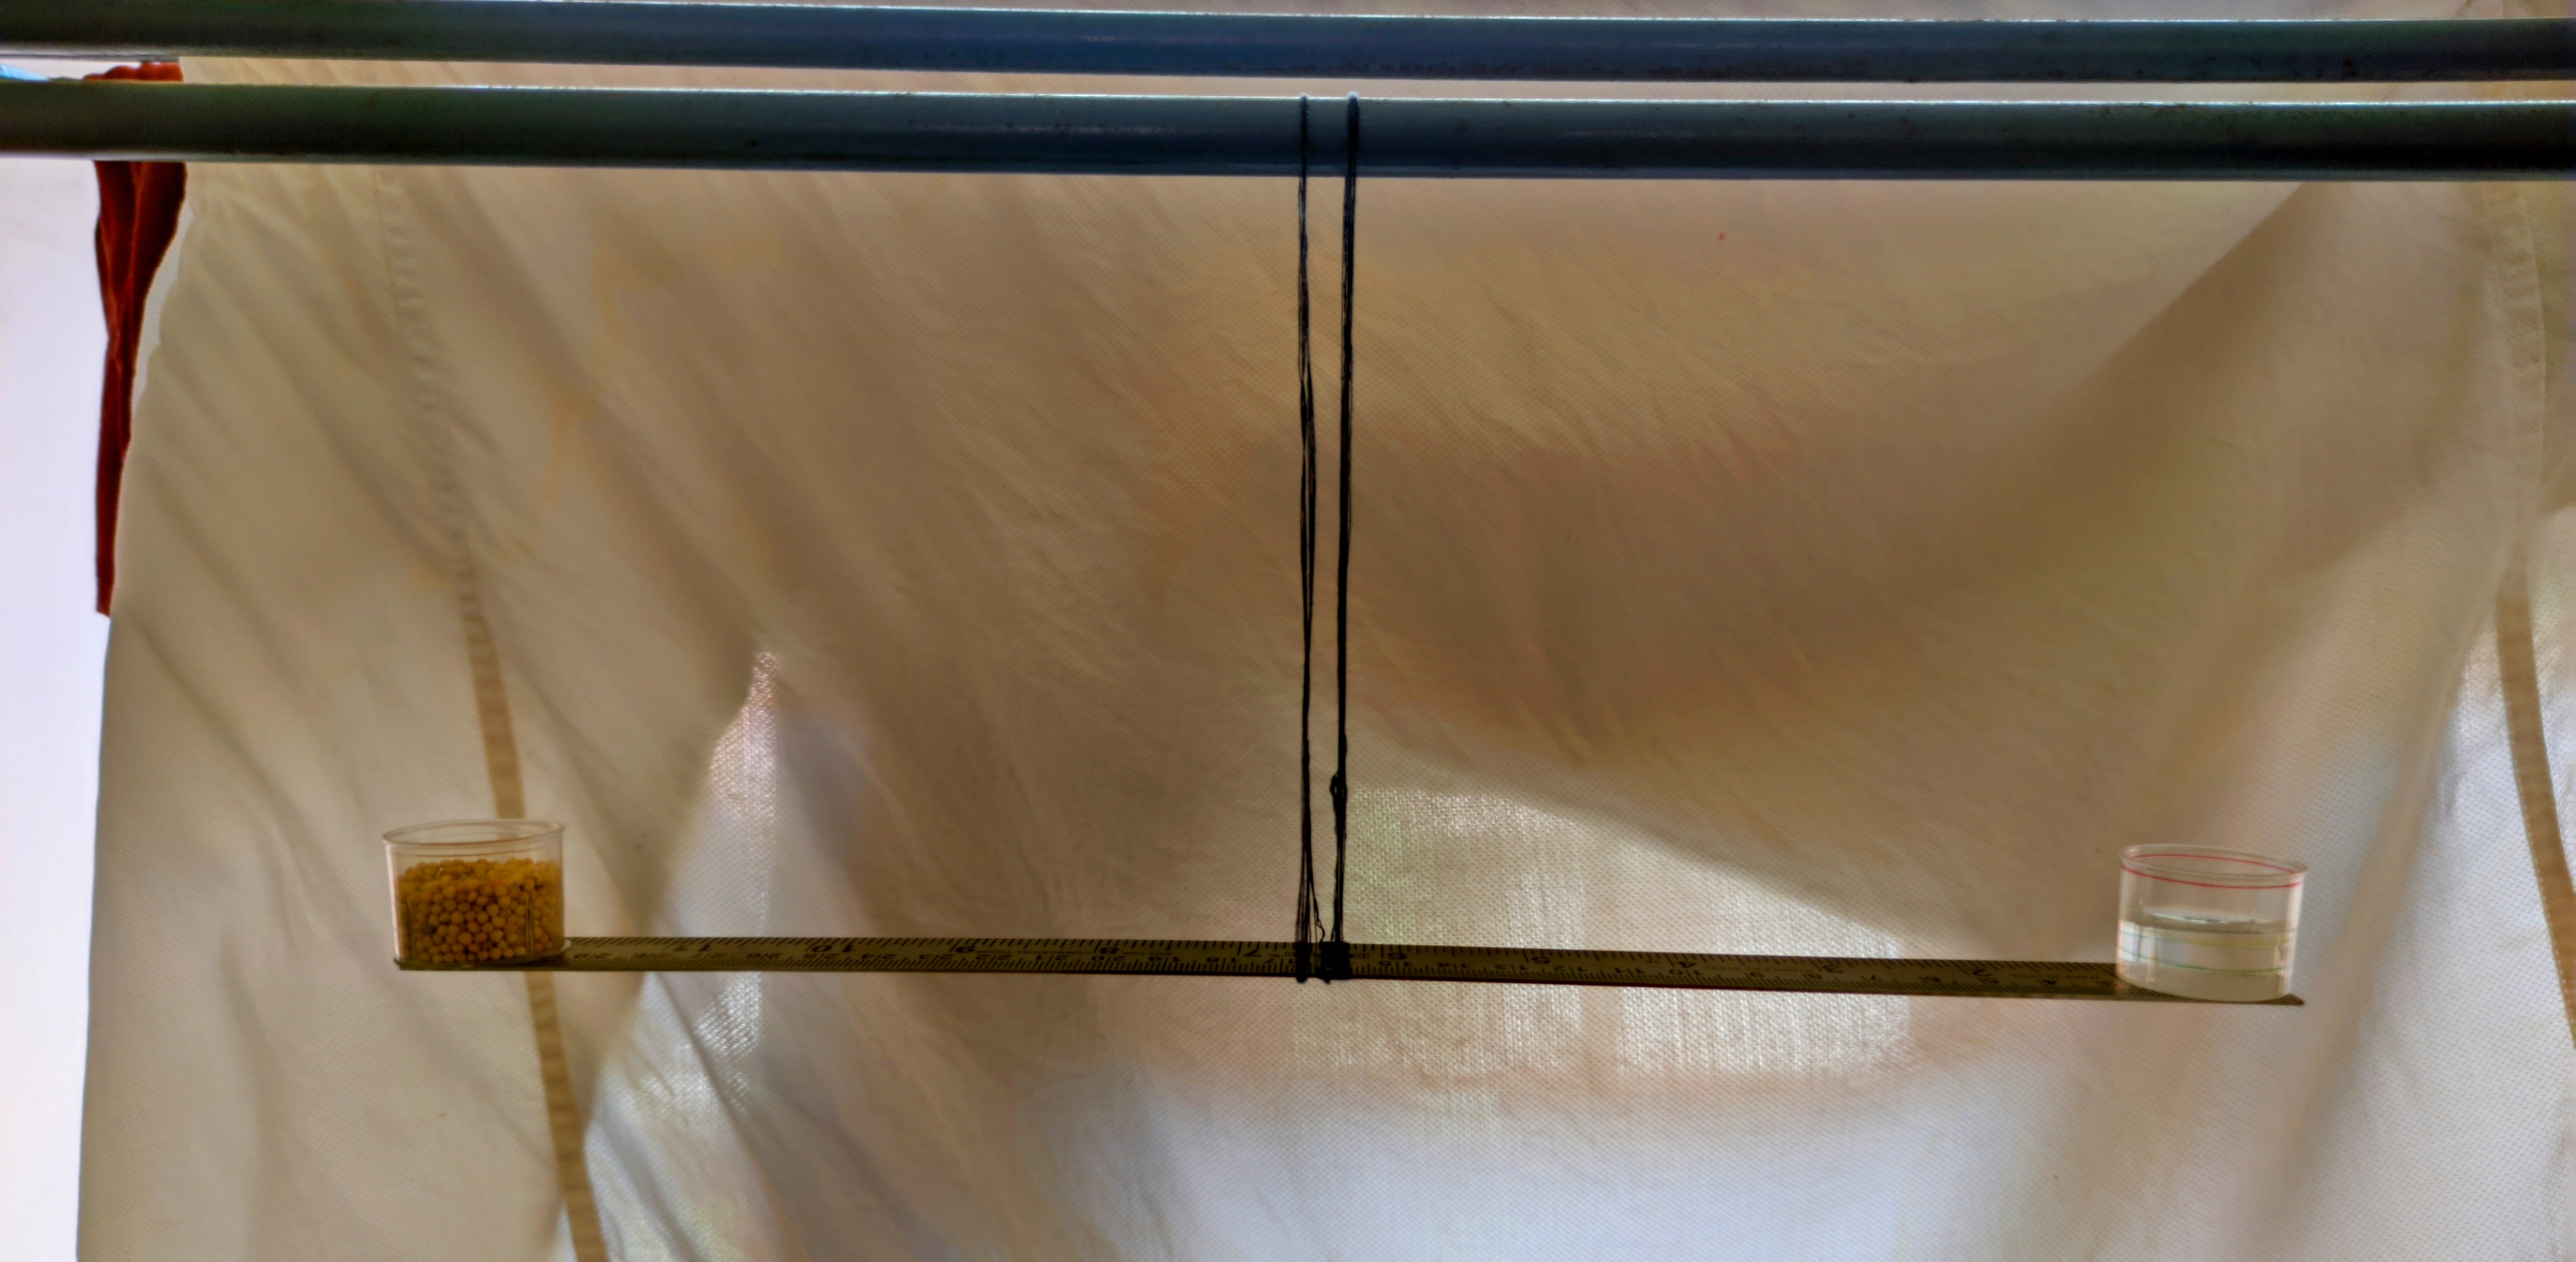
\includegraphics[scale =0.05]{balance_mustard.jpg}
    \caption{Set-up of the beam-balance Click \href{https://drive.google.com/file/d/1gjN0wI8lRWEJ8fQ76qGaELFLVM8-Ln7-/view?usp=drive_link}{here} for the measurement video of the mustard seeds}
    \label{Set-up of the beam-balance}
\end{figure}
    Volume to which the seeds were packed tightly as possible\footnote{Here, I transferred the seeds to another cup with more graduations to get the volume} = 7.5 ml \\    
    Radius of the measuring cup = 1.3cm  \\
   % Volume of the cup =    \\  
    Level to which water was filled = 5ml      \\ 
    Volume of water =    5ml       \\

\subsubsection{Calculations:}

    Density of the seeds = $\rho_s$\\
    Density of water = $\rho_w$\\ = 0.99631 gm/cc (Refer\cite{density_of_water_0-100_Celsius} for more details)\\
    Volume of the seeds = $V_s$ = 7.5ml \\
    Volume of the water = $V_w$ = 5ml\\
   % Mass of the seeds = $m_s$\\
    %Mass of the water = $m_w$\\
    Temperature during the time of the experiment = 28 $\degree$C\\

    Acceleration due to gravity = $g$

    Now, as we know that the weight on both sides are the same,
    \begin{equation}
    \label{Beameq}
        m_sg = m_wg    
    \end{equation}
     
    $$\rho_sV_s = \rho_wV_w$$
    $$\rho_s = \frac{\rho_w V_w}{V_s}$$
    $$\rho_s = \frac{0.99631 \times 5}{7.5} = 0.6642 gm/cc$$

\begin{tcolorbox}[width=8cm,colback={aqua},title={Something looks Fishy!!!},colbacktitle=white,coltitle=black]    
   The experiment in part-2(see \href{https://drive.google.com/file/d/1N1UEq41S4PZ4nuCFbdfE7pa2dK3SC3VD/view?usp=drive_link}{video}) clearly shows that the seeds are sinking, and that means their density must be greater than that of water. So, it can only mean that something less dense than water must be there in between the seeds. Something related to packing...
\end{tcolorbox}

\subsection{Part 2: Measuring Density from Terminal Velocity}
\subsubsection{Data Tabulation of the time intervals of the fall and the Corresponding Terminal Velocity}
Length travelled = height of the Marked interval = 16.5\\
\begin{center}
\begin{tabular}{|p{1cm}||p{3cm}|p{3cm}|} 
 \hline
 SL. No. & Time Required (sec) & Terminal Velocity (cm/sec) \\ [0.5ex] 
 \hline\hline
 1 & 3.850 & 4.286 \\ 
 \hline
 2 & 3.280 & 5.030 \\
 \hline
 3 & 3.261 & 5.059 \\
 \hline
 4 & 3.300 & 5.00 \\
 \hline
 5 & 3.97 & 4.156 \\ 
 \hline
 6 & 3.04 & 5.427\\
 \hline
 7 & 3.42 & 4.824\\
 \hline
 8 & 3.47 & 4.755\\
 \hline
 9 & 3.65 & 4.520\\
 \hline
 10 & 3.68 & 4.483 \\
 \hline
\end{tabular}
\end{center}
 \href{https://drive.google.com/file/d/1N1UEq41S4PZ4nuCFbdfE7pa2dK3SC3VD/view?usp=drive_link}{Click here} for the video demonstration of the experiment

So, the average terminal velocity for the white mustard seeds comes out to be $v_T =4.754 cm/sec.$

\subsubsection{Calculations:}
Temperature during the time of the experiment = 28 $\degree$C\\
viscosity of the water = $\eta$\\ = 	0.008324 poise, using Literature Value \cite{Vis_Lit}
Terminal Velocity of the seeds = $v_T$\\
Acceleration due to gravity(in Kolkata) =  $g= 979.14 dyne/cm^2$\\
Radius of the seeds = $r_{seed}$\\

Now,

\begin{equation}
    \label{Viscousity}
    v_T = \frac{2r_{seed}^2(\rho_{seed} - \rho_{water})g}{9\eta}
\end{equation}

Rearranging we get,

\begin{equation}
\label{density_from_viscousity}
    \rho_{seed} = \frac{9v_{T}\eta}{2g r_{seed}^2} + \rho_{water}
\end{equation}

Putting the required values we get,
 $$\rho_{seed} = 1.0165 gram/cc$$
 
\section{Answering the main Question:}
We will explore the discrepancy between the densities obtained from Part 1 and Part 2 of the experiment. Additionally, we will calculate the packing fraction, which represents the ratio of the actual volume of the spheres to the volume they occupy when packed together.


\subsection{Question: Why is the Density of Seed Obtained Different?}

We got ${\rho_{seed}}_{part-1} = 0.6642 gm/cc$ and ${\rho_{seed}}_{part-2} = 1.0165 gm/cc$, which is about 34.658\% difference with respect to the density from Part-2.
\\
It has to be that in Part-1 as they are hard seeds/spheres, some gaps remain and henceforth, the packing is inefficent as less denser air is also occupying the same volume and henceforth decreasing the overall density of the totality.
\\
In Part-2 as we are using the terminal velocity though with ambiguities of the wall effect and approximation of the point of the terminal velocity being reached, it gives a value which at least satisfies the condition of the seeds being denser than water at the same temperature, and so is much closer to the reality.

In all, the differnce in the densities will help us get the packing fraction of the small white mustard seeds.
\subsection{So, then how much does the mustard actually pack?}

The packing fraction(PF) from the two experiments can be calculated as follows:
\begin{equation}
\label{pf}
    PF = \frac{{Volume_{seed}}_{part-1}}{{Volume_{seed}}_{part-2}} 
\end{equation}

$=\frac{{\rho_{seed}}_{part-1} m_seed}{{\rho_{seed}}_{part-2}m_seed} = 0.6534$

So, in the part-1 experiment only 65.34\% of the 7.5ml volume was actually mustard seed material.

\section{Extra Exploration}
\subsection{Adding on the same experiment:}
\subsubsection{Getting the packing fraction from the Radius and number of seeds:}

Refer \eqref{Volume of the seeds in the cup}, and using this 4.823ml volume covered by 1343 mustard seeds, with respect to the 7.5ml of the apparent volume, let's find the packing fraction,

refer \eqref{pf}, 
putting the required values we get,
$$PF = \frac{4.823}{7.5} = 0.64306$$

Hnece, here we got a packing efficiency of 64.306\%.


\begin{comment}
    
\subsubsection{Re-checking the Radius:}
At the terminal velocity, the acceleration is zero, and Newton's second law gives
\beq
0=6\pi r \eta v_T +\frac{4}{3}\pi r^3 \rho_{water} g - \frac{4}{3}\pi r^3 \rho_{seed} g
\label{eq:freefall}
\eeq
where $v_T$ is the speed of the seed moving downward.

Equation \ref{eq:freefall} can be solved for the radius of the seed;
\beq
\label{Recheck radius}
r=\sqrt{\frac{9\eta v_T}{2(\rho_{seed}-\rho_{water})g}}
\label {eq:radius}
\eeq

\end{comment}

 \subsubsection{How about 2D Packing:}
 Radius of the medicine cup used = 1.3cm \\
 Number of the seeds =    177      \\
 Average radius of each seed =  0.095cm    \\
 Area of the cup base = $\pi R_{cup} ^2$ = 5.31 cm^2     \\
 Area covered by the 177 seeds = $177\pi R_{seed}^2= 5.018cm^2$\\
 So, packing fraction = 
 \begin{equation}
     \label{PF_2D}
    PF = \frac{\text{Area Covered by Seeds}}{\text{Area of the Cup Base}}
 \end{equation}
 $$ &= \frac{5.018}{5.310}= 0.945$$

So, these white mustard seeds while considering their mean radius (see \href{https://drive.google.com/file/d/106FkTC_GaYkQ8QXoM8jGT479VFAHoQ2f/view?usp=drive_link}{here}), have a 2D packing efficiency of about 94.5\%.
 
\subsection{Extra Experiment with Black pepper:}
The same procedure was followed for the black pepper\footnote{which I was able to procure from our canteen. I thank our mess workers for being generous.}, and so, I am directly jumping on with the tabulation and calculations.

\subsubsection{Radius Data Table}
\begin{center}
\begin{tabular}{||c | c | c ||} 
 \hline
 SL. No. & Diameter (cm) & Radius (cm) \\ [0.5ex] 
 \hline\hline
 1 & 0.4 & 0.2 \\ 
 \hline
 2 & 0.5 & 0.25 \\
 \hline
 3 & 0.4 & 0.2 \\
 \hline
 4 & 0.5 & 0.25 \\
 \hline
 5 & 0.5 & 0.25\\ 
 \hline
 6 & 0.5 & 0.25 \\
 \hline
  7 & 0.6 & 0.3 \\
 \hline
 8 & 0.5 & 0.25 \\
 \hline
 9 & 0.4 & 0.2 \\
 \hline
 10 & 0.5 & 0.25 \\
 \hline
\end{tabular}
\end{center}
\\
So, Average Radius of black pepper is $R_s &=  0.24 cm$\\
Number of seeds here = 93 \\

So, volume occupied by 93 seeds = 
\beq
\label{Volume of the pepper seeds in the cup}
93\frac{4}{3}\pi R_s^3 = 5.385 ml
\eeq

\subsubsection{Data from Beam Balance}
    Click \href{https://drive.google.com/file/d/16dkCRaP8JWYyElnq-B_HgopsTJ5laUmY/view?usp=drive_link}{here} for the video of the experiment\\
    Volume to which the seeds were packed tightly as possible = 10 ml\\
    Radius of the measuring cup = 1.3cm  \\
    %Volume of the cup =    \\  
    Level to which water was filled = 5ml      \\ 
    Volume of water =  5ml         \\
\subsubsection{Calculations:}
    Refer \eqref{Beameq}
    $$\rho_sV_s = \rho_wV_w$$
    $$\rho_s = \frac{\rho_w V_w}{V_s}$$
    $$\rho_s = \frac{0.99631 \times 5}{10} = 0.498 gm/cc$$

\subsubsection{Data Tabulation of the time intervals of the fall and the Corresponding Terminal Velocity}
\begin{figure}[H]
    \centering
    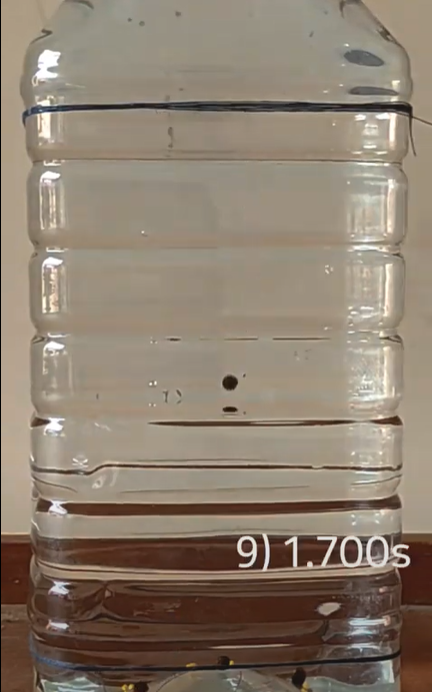
\includegraphics[scale= 0.5]{Terminal_pepper.png}
    \caption{A snapshot of the experimental setup i.e. a plastic jar\protect\footnotemark during runtime}
    \label{A snapshot of the experimental setup during runtime}
\end{figure}
Length travelled = height of the Marked interval = 16.5cm\\


    \footnotetext{I got this from a local bakery. I thanks that guy for lending me this jar.}
\begin{center}
\begin{tabular}{|p{1cm}||p{3cm}|p{3cm}|} 
 \hline
 SL. No. & Time Required (sec) & Terminal Velocity (cm/sec) \\ [0.5ex] 
 \hline\hline
 1 & 1.930 & 8.549 \\ 
 \hline
 2 & 1.950 & 8.461 \\
 \hline
 3 & 1.900 & 8.684 \\
 \hline
 4 & 2.110 & 7.819 \\
 \hline
 5 & 1.619 & 10.191 \\ 
 \hline
 6 & 1.520 & 10.855\\
 \hline
 7 & 1.670 & 9.880\\
 \hline
 8 & 1.800 & 9.167\\
 \hline
 9 & 1.7 & 9.706\\
 \hline
 10 & 1.61 & 10.248 \\
 \hline
\end{tabular}
\end{center}
 \href{https://drive.google.com/file/d/1zuYuvHTLJAr_wVvc-JMsfif2ErYpfE5w/view?usp=drive_link}{Click here} for the video demonstration of the experiment.\footnote{Due to the coarse and even surface of the peppercorns, they always tried to create air pockets and thus increasing the bouncy which lowers the terminal velocity. I tried my best by first getting them wet for a few seconds before dropping them.}

So, the average terminal velocity for Black peppercorns is $v_T &= 9.356 cm/s$


\subsubsection{Calculations:}
Temperature during the time of the experiment = 28 $\degree$C\\
viscosity of the water = $\eta$\\ = 	0.008324 poise, using Literature Value \cite{Vis_Lit}
Terminal Velocity of the seeds = $v_T$\\
Acceleration due to gravity(in Kolkata) =  $g= 979.14 dyne/cm^2$\\
Radius of the seeds = $r_{seed}$ =0.24cm\\

Now,\\
Refer \eqref{Viscousity} and \eqref{density_from_viscousity},
\\
Putting the required values we get,
 $${\rho_{seed}}_{black-pepper} = 1.00252 gram/cc$$
 
\subsubsection{The Packing fraction from density difference}
Refer \eqref{pf},
So, using the density difference from the two parts we get the final packing fraction as,
$$PF = \frac{0.498}{1.00252}= 0.4967$$

From this method, the black peppercorns have a packing efficiency of only 49.67\%.

\subsubsection{The Packing Fraction from Radius and Number of seeds:}
Refer \eqref{Beameq}, and using this 5.385ml volume covered by 93 black peppercorns, with respect to
the 10ml of the apparent volume, let’s find the
packing fraction,
refer \eqref{pf}, putting the required values we get
$$PF = \frac{5.385}{10} = 0.5385$$
So, from this way, we got a packing efficiency of about 53.85\% for black peppercorns.
\subsubsection{Let's do the 2D packing again}
Refer \eqref{PF_2D},\\
Knowing that the same measuring cup was used, so the base area of the cup is still $5.31 cm^2$\\
Now, the number of peppercorns = 23
so,

$$PF_{2D} = \frac{23\pi R_{black pepper}^2}{\pi R_{cup}^2}= 0.7839$$

Click \href{https://drive.google.com/file/d/1s73ig5K-jH7DYv54-HVJCJj_UxN6Z78_/view?usp=drive_link}{here} to see the packing and here it comes out to be about 78.39\%

\subsection{Some Theorical Points to be added:}

In actual practice, the experiment is performed in a liquid column of finite depth $h$(refer \eqref{Illustrative Diagram for the Part-2 Experiment} contained in a cylinder of inner radius $R$. To take into account the effect of the finite depth and radius of the liquid column, two corrections, known as Ladenburg corrections, are introduced as multipliers of the observed velocity $v'$. Thus, the terminal velocity $v$ is given by
\begin{equation}
\label{Ladenburg}
v = v' \left(1+ \frac{2.4r}{R} \right) \left( 1+ 3.33\frac{r}{h} \right),
\end{equation}
where the first correction term accounts for the finite radius of the liquid column and the second correction term is used for the finite depth of the liquid column. 

\begin{tcolorbox}[width=8cm,colback={aqua},title={Remark about the Correction terms:},colbacktitle=white,coltitle=black]   
Since I used thin plastic jars, the $\frac{r}{R}$ term is quite negligible but the height of the jar is not. So, the calculations given in this context can easily be re-calculated while keeping in mind the corrections.
Refer \cite{H_Brenner} for more details.
I couldn't find the original paper (refer \cite{LADENBURG}). But I did mention his correction terms.
\end{tcolorbox}



\section{Error Analysis :}
\subsection{Theoritical Error Analysis:}

    We need to note that the errors are here only with respect to the least count of the instrument used, so, the error of the $\rho_{seed}$ will be different for Part-1 and Part-2 respectively.
    \\
    In Part -1, using the beam balance, we got,\\
    \begin{equation}
    \label{error_part-1}
        \frac{\Delta \rho_{seed}}{\rho_{seed}}|_{Part-1} &= 3\frac{\Delta r_{cup}}{r_{cup}} + 3\frac{\Delta r_{seed}}{r_{seed}} +\frac{\Delta \rho_{water}}{\rho_{water}}
    \end{equation}
    \\
    Knowing,
$$\Delta r = 0.05cm$$
$$r_{mustard} = 0.095cm$$
$$r_{black pepper}=0.24$$
$$r_{cup} = 1.3cm$$
We are using literature value\cite{density_of_water_0-100_Celsius} for density of water. 
    Putting the least count values scaled for the radius and the measured values in \eqref{error_part-1}, we get
    
    $$\frac{\Delta \rho_{seed}}{\rho_{seed}}|_{Part-1} = \frac{0.05}{1.3} + \frac{0.05}{0.095}=1.694$$

    This humungous error is true as we already disclosed the packing fraction story.
    But another thing to note is that the values measured are very close to the least count of the device and hence we are getting such high uncertainities.\\
Now, for the black pepper one we get,
    
    $${\frac{\Delta \rho_{seed}}{\rho_{seed}}|_{Part-1}}_{black pepper} = \frac{0.05}{1.3} + \frac{0.05}{0.24}=0.740$$


    
    From \eqref{Viscousity} we can get the error expression by taking log and then differenciating while knowing that error is non-compensative in this experiment,
We know,
$$\Delta v_T = 0.1 cm/sec$$\dots as it depends on the significant digits of the metal scale\\
$$\Delta r_{seed} = 0.05cm$$
$${v_T}_{mustard} = 4.754 cm/sec$$
$${v_T}_{black pepper} = 9.356 cm/sec$$
Both the density and viscosity of water terms were from Literature\cite{density_of_water_0-100_Celsius}\cite{Vis_Lit}, and also the same for acceleration due to gravity..
    
\begin{equation}
\label{error_part2}
    \frac{\Delta\rho}{\rho}|_{mustard} =
    \frac{\Delta\rho_{water}}{\rho_{water}} + \frac{\Delta v_{T}}{v_{T}} + \frac{\Delta\eta}{\eta} + 2\frac{\Delta r_{seed}}{r_{seed}}+ \frac{\Delta g}{g}
\end{equation}

$$= \frac{0.1}{4.754} +2\frac{0.05}{0.095}=1.073$$

Using \eqref{error_part2} for black pepper we get the error as,

$${\frac{\Delta\rho_{seed}}{\rho_{seed}}}_{black pepper}=\frac{0.1}{9.356} +2\frac{0.05}{0.24}=0.427$$


Again, the measurement of the radius being so close to the least count creates trouble.


\subsection{Relative Error Calculation wrt Literature Values:}
We know that for white mustard seeds "true density 1.169 g cm-3 ('Warta') and 1.203 g cm-3 ('Radena')"\cite{mustard_data}.
Here, the variety used is Warta.
So, using this value as the most accurate one, let's find the relative with the density we got from the part-2 experiment.



$$\text{Relative Error \%} =$$
\begin{equation}
\label{Relative_Error}
\frac{|Observed Value-Literature Value|}{Literature Value} \times 100 \%
\end{equation}
$$= 13.04\%$$

Now, for the black peppercorns, "The true density increased linearly as a function of moisture from 987.7 to 1012.2 $kgm^{-3}$"\cite{pepper_data}. \\
Since it is monsoon season here with daily rainfall, I shall be considering the max limit and again if you look in the video, I was also dipping the peppercorns before dropping them as they had an uneven surface which leads to air pockets being formed. 
\\Refer \eqref{Relative_Error},
$$\text{Relative Error \%} = \frac{|1.0122-1.00252|}{1.0122} \times 100\%$$
$$=0.95\%$$

\section{Observations, Inferences and Understandings}

\begin{enumerate}
    \item \textbf{Particle Property Analysis:} The experimental study focused on the analysis of white mustard seeds and black pepper seeds as representatives of minute particles. The two measurement methodologies employed successfully provided valuable insights into the mass, density, and volume characteristics of these tiny seeds.
    
    \item \textbf{Measurement Discrepancies:} Discrepancies observed in the density measurements between the two methodologies were attributed to the presence of inter-seed gaps and less dense air within the measuring setup. These discrepancies emphasize the challenges in accurately measuring the properties of such minute particles.
    
    \item \textbf{Packing Fraction and Efficiency:} The packing fraction of white mustard seeds was determined to be approximately 65.34\%, with a packing efficiency of 64.306\% based on the seed radius and quantity. The 2D packing analysis resulted in a higher efficiency of 94.5\%. Similarly, black pepper seeds exhibited a packing efficiency of 49.67\% based on density variations, and a packing efficiency of 53.85\% considering the seed radius and number. The 2D packing analysis for black pepper seeds yielded an efficiency of 78.39\%.
    
    \item \textbf{Comparative Analysis:} The study provides a comparative analysis of the packing efficiencies of white mustard and black pepper seeds. The results indicate that white mustard seeds have higher packing efficiency compared to black pepper seeds, suggesting differences in their particle arrangements.
    
    \item \textbf{Significance of Measurement Techniques:} The experiments highlight the importance of employing appropriate measurement techniques for accurate analysis of minute particles. It underscores the need for refined methods to overcome challenges in obtaining precise data from such small-scale specimens. Refer Ladenburg\cite{H_Brenner}'s correction terms which have been further improved by H. Brenner.
    
\end{enumerate}
\section{Conclusion}
This study elucidates the particle packing efficiency of white mustard and black pepper seeds, highlighting the significant impact of seed morphology on attainable packing fractions. The intricate relationship between particle size, shape, and interlocking mechanisms is evident, underscoring the importance of understanding granular materials at a fundamental level.

\bibliographystyle{abbrvurl}
\bibliography{ref}
\end{document}